\documentclass[../EngineeringJournal_CDavis.tex]{subfiles}

\begin{document}

%%%%%%%%%%%%%%%%%%%%%%%%%%%%%%%%%%%%%%%%%%%%%%%%%%%%%
%%%%%%%%%%%%%%%%%%%%%%%%%%%%%%%%%%%%%%%%%%%%%%%%%%%%%

\chapter[Troubleshooting Vlan]{Troubleshooting Vlans\linebreak[1] Scenario 1
\hspace*{\fill February 29, 2020}}
\noindent\textbf{{Netlab Lab 11} \hspace*{\fill}{\textbf{CIT 167}}}\linebreak[1]
{{Spring 2020} \hspace*{\fill}{Chaz Davis}}                             
%===================================
%===================================


\hspace{0.2cm}
\begin{tcolorbox}[width=6.3in]
\scriptsize 
troubleshooting vlans
  \begin{outline}
    \1 something something blah
  \end{outline}
\end{tcolorbox}
\hspace{0.2cm}
\normalsize  
  
\clearpage

%===================================
\mysection{\textbf{Part 1: Test Connectivity between PCs on the Same VLAN}}

\mysubsection{1}{Can PC1 ping PC4}
\\Attempt to ping PC4 from PC1 was unsuccessful. See
Fig.~\ref{Ping11}~\subref{Ping11PC1}. 

\noindent\mysubsection{2}{Can pc2 ping pc5}
\\Attempt to ping PC5 from PC2 was unsuccessful. See
Fig.~\ref{Ping11}~\subref{Ping11PC2}. 

\noindent\mysubsection{3}{Can pc3 ping pc6}
\\Attempt to ping PC6 from PC3 was unsuccessful. See
Fig.~\ref{Ping11}~\subref{Ping11PC3}. 


\begin{figure}[!hbt]\centering
\subfloat[PC1 pinging
PC4]{\label{Ping11PC1}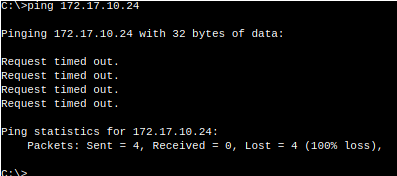
\includegraphics[width=.45\linewidth]{Figures/2020-03-08-001241_397x176_scrot.png}}\par
\subfloat[PC2 pinging
PC5]{\label{Ping11PC2}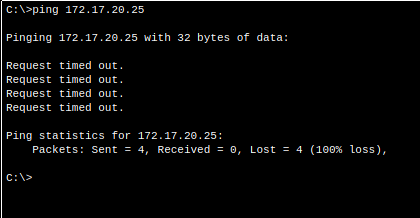
\includegraphics[width=.45\linewidth]{Figures/2020-03-08-001302_420x218_scrot.png}}\hfill
\subfloat[PC3 Pinging
PC6]{\label{Ping11PC3}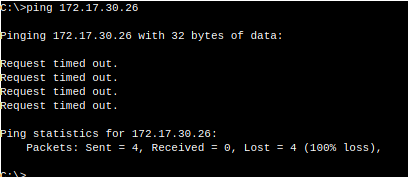
\includegraphics[width=.45\linewidth]{Figures/2020-03-08-001401_408x177_scrot.png}}\par
\caption{Testing Connections on the same networks}
\label{Ping11}
\end{figure}




%===================================
\mysection{\textbf{Part 2: Investigate Connectivity Problems by Gathering Data}}

\mysubsection{1}{Verify Configurations on the PCs}
\\I checked configurations for IP address and subnetmasks on all pcs. 
PC5 had an incorrect IP address.

\noindent\mysubsection{2 \& 3}{Verify Configs on the Switches}
\\On switch2 vlan for subnet 30 had the 10 and 30 subnets attached to it, so I
moved the Fa0/11 interface to 10 faculty/staff. Also on S2, G0/1 was not setup
as a trunk.

PC5 appears to be connected on port Fa0/17 when it should be Fa0/18.

Switch3, vlan 20 and vlan 30 are switched on their connections.


%===================================
\mysection{\textbf{Part 3: Implement the Solution and Test Connectivity}}

On S2 I ran {\scriptsize{\verb$int fa 0/11$}\normalsize} and then
{\scriptsize{\verb$switchport access vlan 10$}\normalsize}to correct the first
issue.
Then I ran, {\scriptsize{\verb$int g0/1$}\normalsize} and then
{\scriptsize{\verb$switchport mode trunk$}\normalsize}. 

On S1, I ran {\scriptsize{\verb$int g0/1$}\normalsize} and then
{\scriptsize{\verb$switchport mode trunk$}\normalsize}.

On S3, I ran {\scriptsize{\verb$int f0/18$}\normalsize} and then
{\scriptsize{\verb$switchport access vlan 20$}\normalsize}.
I then ran {\scriptsize{\verb$int f0/6$}\normalsize} and then
{\scriptsize{\verb$switchport access vlan 30$}\normalsize}.

I'll now attempt to ping each of the connected networks.
All pings were successful. See Fig.~\ref{Success11}.


\begin{figure}[!hbt]\centering
\subfloat[PC1 pinging
PC4]{\label{Success11PC1}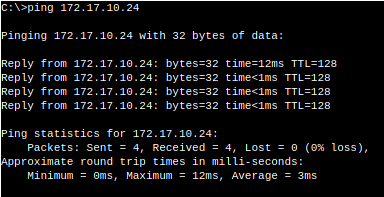
\includegraphics[width=.45\linewidth]{Figures/2020-03-08-074940_384x197_scrot.png}}\par
\subfloat[PC2 pinging
PC5]{\label{Success11PC2}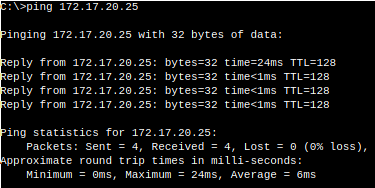
\includegraphics[width=.45\linewidth]{Figures/2020-03-08-074950_375x188_scrot.png}}\hfill
\subfloat[PC3 pinging
PC6]{\label{Success11PC3}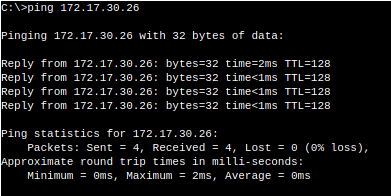
\includegraphics[width=.45\linewidth]{Figures/2020-03-08-075000_391x196_scrot.png}}\par
\caption{Network connections are now all successfull}
\label{Success11}
\end{figure}



\begin{figure}[!hbt]\centering
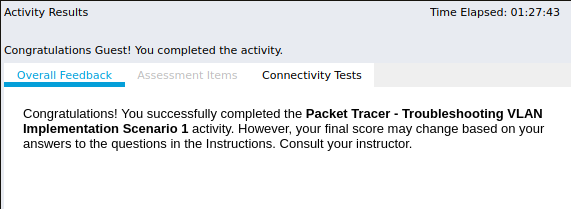
\includegraphics[width=.45\linewidth]{Figures/2020-03-08-075242_571x209_scrot.png}
\caption{Successful Completion of the Activity}
\label{Complete11}
\end{figure}

%===================================

\end{document}
